\chapter{Disjoint path in decomposable digraphs}
\label{chap:linkage}
In this chapter we will cover the Linkage problem given a set a decomposable digraph $D$ and a set of terminals $\Pi$ to be linked. 
We will explaining the problem and shortly show why the problem is interresting (NP-complete). 
After this we will in \autoref{sec:lQuasi} show that the linkage problem is polynomial solveable in $\phi$-decomposable digraph as long as $\phi$ is a linkage ejector after that we will show that $\phi_1$ is a linkeage ejector meaning that the linkage problem is solveable for quasi-transitive digraphs(all of this is only true if the number of pairs needed linking is fixed). Then in \autoref{sec:lLocally} we will cover the 3 different subclasses a locally semicomplete digraph can be a part of, and solve the $k$-linkage problem for those in polynomial time for a fixed $k$. 
\section{The Linkage Problem}
\label{sec:lNP}
Given a digraph $D$ and two distinct vertices $s$ and $t$ we want to make a path from $s$ to $t$ denoted this $P$. 
Recall that in this case $s$ will be the source of $P$ and $t$ the zink.
Now let $s_1,t_1,\dots ,s_k,t_k$ be distinct vertices of $D$, then the \textbf{$k$-linkage} problem is to decide if there exists paths $P_1,\dots ,P_k$ linking the vertices so $P_i$ link the pair $(s_i,t_i)$ $\forall i\in [k]$ and each path $P$ has to be vertex disjoint from the others. This problem is also somtimes just called \textbf{the linkage problem}.
The problem is actually NP-complete already when $k=2$, so we will be focusing on the problem when $k$ is fixed.
%This we sould be able to do easily if one exists, but when adding two extra distict vertices $u$ and $v$ not nessesarily distinct from $s$ and $t$ and we want a path $Q$ between $u$ and $v$ distinct from the path $P$ the problem suddenly become NP-complete.
The vertices $s_1,t_1,\dots , s_k,t_k$ are called \textbf{terminals} and $(s_1,t_1);\dots ;(s_k,t_k)$ are called \textbf{terminal pairs}.
The notation for this problem in this thesis would be using $k$ as the natural number of pairs of terminals, and the set of these terminals is denoted $\Pi=\lbrace (s_1,t_1);\dots ;(s_k,t_k)\rbrace$. 
As we have done optil now we will still use $D$ as the main digraph we are looking at unless anything else is specified. 
$L$ is used as a collection of paths $P_1,\dots , P_l$ if $L$ is the solution to our linkage problem it means $l=k$ and the path $P_i$ links the pair $(s_i,t_i)$ for all $i\in [k]$.
If $L$ upholds the above conditions we say that $L$ is a $\Pi$-linkage, or $L$ is the linkage of $(D,\Pi)$.\\
Recall that a quasi-transitive digraph is build up by either a transitive acyclic digraph or semicomplete digraph as the quotient of the decomposition. 
And for these to classes of digraph we kan solve the $k$-linkage problem in polynomial time for a fixed $k$. With fixed $k$ there means that an algorithm given a digraph and a naturel number $k$ can solve the $k$-linkage problem(it is possible that the algorithm needs more information). When $k$ is not fixed then it is already NP-complete for tournaments, since tournaments is a very strict class we will only focus on when $k$ is fixed.


\section{Solving the Linkage Problem in $\phi$-decomposable Digraphs}
\label{sec:lQuasi}
From \autoref{thm:quasidecom} we know that a quasi-transitive digraph is a composition of acyclic transitive digraphs and semicomplete digraphs.
We know that $\phi_1$ is the union of acyclic and semicomplete digraphs, which means that every quasi-transitive digraphs are $\phi_1$-decomposable as described in \autoref{chap:decomposable}. 
\begin{thm}~\cite{bangJGT85}
    For every fixed $k$, there exists a polynomial algorithm for the $k$-linkage problem on acyclic digraphs.
\end{thm}
\begin{thm}
    For every fixed $k$, there exists a polynomial algorithm for the $k$-linkage problem on semicomplete digraph.
\end{thm}
Note that this means that there exists polynomial algorithms for a fixed $k$ to solve the $k$-linkage problem for digraphs in $\phi_1$.\\
For a decomposition $D=S[M_1,\dots M_s]$ and a set of terminal pairs, we can split the set into two different sets of terminals. 
The set of \textbf{internal pairs} $\Pi_i$, where internal pair means that both $s_i$ and $t_i$ is in the same hause, and the set of \textbf{external pairs} $\Pi_e$ which is the rest such that $\Pi=\Pi_i \cup \Pi_e$.\\
\begin{lemma}~\cite{bangJGT85}
    Let $D=S[M_1,\dots ,M_s]$ be a decomposable digraph and $\Pi$ a set of pairs of terminals. Then $(D,\Pi)$ has a linkage if and only if it has a linkage whose external paths do not use any arc of $D\left<M_i\right>$ for $i\in [s]$.
\end{lemma}
\begin{proof}
    \textcolor{red}{blablabalbalbalab}
\end{proof}
Meaning that the external paths do not use arcs inside the hauses only arcs to come from house to house (arcs from the quotient digraph $S$). Be aweare that internal pairs can be linked by an internal path or an external path going out of the house and later in agian, where ofcourse external pairs has to be linked by external paths. 

Before getting into the algorithm for solbing this for $\phi$-decomposable digraphs, we need to set some conditions for the set $\phi$. 
When a set of digraphs $\phi$ upholds these conditions we are going to say that $\phi$ is a linkage ejector. 
But first we need to establish that a set of digraphs can be closed with respect to blow-up.
\textbf{blow-up} means blowing up a vertex $v$, with a digraph $K$(Replacing $v$ with the digraph $K$).
When a set of digraphs $\phi$ is closed with respect to this operation it means that for a digraph $D\in \phi$ there exists a digraph $K$ such that after $K$ has replaced $v$ the digraph is still a part of the set $\phi$. 
This definition brings this nice lemma.

\begin{lemma}
    If a class $\phi$ is closed with respect to the blowing-up operation $S\in \phi$ and $D=S[M_1,\dots M_s]$, then it is possible to replace the arcs in the digraph $M_i$ with other arcs, so that the resulting digraph is in $\phi$. 
    \label{lemma:replace} 
\end{lemma}

This brings us to the definition of a linkage ejector.
\begin{definition}~\cite{bangJGT85}
    A class of digraphs $\phi$ that is closed with respect to blow-up is a linkage ejector if the following conditions is true
    \begin{enumerate}
        \item There exists a polynomial algorithm $\mathcal{A}_{\phi}$ to find a total $\phi$-decomposition of every totally $\phi$-decomposable digraph.
        \item There exists a polynomial algorithm $\mathcal{B}_{\phi}$ for a fixed $k$, for solving the $k$-linkage problen on $\phi$
        \item There exists a polynomial algorithm $\mathcal{C}_{\phi}$ that given a totally-decomposable digraph\\ $D=S[M_1,\dots , M_s]$ constructs a digraph of $\phi$ by replacing the arcs inside each $M_i$ for $i\in [s]$ as in \autoref{lemma:replace}. 
    \end{enumerate}
\end{definition}

\textcolor{red}{Algorithm here}

\subsection{linkage for qausi-transitive digraph among other}


\section{Solving Linkgae Problem in Locally Semicomplete Digraphs}
\label{sec:lLocally}
A locally semicomplete digraph is either round decomposable, semicomplete or neither.
We have in \autoref{sec:locally} called these evil locally semicomplete digraph or just evil.
The semicomplete part is solved from \autoref{thm:semiklink} but the theorem will also be important in this section.
First we will look at the evil semicomplete digraph where we need to recall \autoref{thm:evildecom} $(a)$ where we can see that an evil semicomplete digraph can be partitioned into into maximum 4 semicomplete digraphs $S,D_1',D_2',D_3'$ which lead us to the next theorem.
\begin{thm}~\cite{chudnovskyJCT135}
    For every fixed pair of positive integers c,k there exists a polynomial algorithm for the $k$-linkage problem on digraphs whose vertex set is partinionable into $c$ sets inducing semicomplete digraphs.
    \label{thm:inducesemi}
\end{thm}
Let $c=4$ in \autoref{thm:inducesemi}. 
Then we know from \autoref{thm:evildecom} that every evil locally semicomplete digraph has a polynomial algorithm for the $k$-linkage problem when $k$ is fixed.\\

The remaning class of digraphs inside the class of locally semicomplete digraphs is the class of round decomposable digraphs. 
Recall the class $\phi_2=\lbrace\text{semicomplete digraphs}\rbrace\cup\lbrace\text{round digraphs}\rbrace$ from \autoref{sec:gdecomposable}.
As we did in \autoref{sec:lQuasi}, we will in the end prove that $\phi_2$ is a linkage ejector and since round decomposable digraphs are totally $\phi_2$-decomposable, we would have proven that there exists a polynomial algorithm for them.
To prove that $\phi_2$ is a linkage ejector, we know from \autoref{def:ejector} that it needs 3 algorithms $\mathcal{A}_{\phi_2},\mathcal{B}_{\phi_2}$, and $\mathcal{C}_{\phi_2}$. For the algorithm $\mathcal{B}_{\phi_2}$ we only need it for round digraphs.
\begin{thm}
    For every fixed $k$, there exists a polynomial algorithm to solve the $k$-linkage problem on round digraphs.
    \label{thm:roundklink}
\end{thm}
\begin{proof}
    $D$ is round so let $v_1,\dots ,v_n$ be the round ordering and $\Pi = \lbrace (s_1,t_1), \dots (s_k,t_k)\rbrace$ the set of pairs of terminals.
    Given $j\in [n-1]$, we say that an arc $v_av_b$ is \textbf{over} another arc $v_jv_{j+1}$ if $v_b\in \lbrace v_j+1,\dots v_{a-1}\rbrace$. 
    We are now going to show that for a $(s_i,t_i)$-path, it only needs to use one arc over $v_jv_{j+1}$. 
    Let us assume this is not the case and that the $(s_i,t_i)$-path uses two arcs over $v_jv_{j+1}$. 
    Call these two arcs $u_1w_1$ and $u_2w_2$. 
    There are four ways these vertices can be placed in relation to each other in the ordering and still be arcs over $v_jv_{j+1}$. See figure \autoref{fig:cases}.
    \begin{figure}
        \begin{subfigure}[b]{0.49\textwidth}
            \centering
            \begin{tikzpicture}
            %nodes
            \begin{scope}
                \node[draw=none] (u1) {$u_1$};
                \node[draw=none,right = of u1] (u2) {$u_2$};
                \node[draw=none,right = of u2] (w1) {$w_1$};
                \node[draw=none,right = of w1] (w2) {$w_2$};
            \end{scope}
        
            %crosses
            \begin{scope}[very thick,decoration={
                markings,
                mark=at position 0.5 with {\arrow{>}}}
                ] 
                \draw[postaction={decorate},red] (u1)--(u2);
                \draw[postaction={decorate},red] (u2)--(w1);
                \draw[postaction={decorate},red] (w1)--(w2);
            \end{scope}
        
            \begin{scope}
                \path [-{Latex[length=3mm]}] (u1) edge[bend left=30] node[left] {} (w1);
                \path [-{Latex[length=3mm]}] (u2) edge[bend left=30] node[left] {} (w2);
            \end{scope}
            \end{tikzpicture}
        \caption{Case 1}
        \end{subfigure}
        \begin{subfigure}[b]{0.49\textwidth}
            \centering
            \begin{tikzpicture}
            %nodes
            \begin{scope}
                \node[draw=none] (u2) {$u_2$};
                \node[draw=none,right = of u2] (u1) {$u_1$};
                \node[draw=none,right = of u1] (w1) {$w_1$};
                \node[draw=none,right = of w1] (w2) {$w_2$};
            \end{scope}
            
            %crosses
            \begin{scope}[very thick,decoration={
                markings,
                mark=at position 0.5 with {\arrow{>}}}
                ] 
                \draw[postaction={decorate},red] (u2)--(u1);
                \draw[postaction={decorate},red] (w1)--(w2);
                \draw[postaction={decorate},red] (u2) to [bend right] (w1);
                \draw[postaction={decorate},red] (u1) to [bend right] (w2);
            \end{scope}
            
            \begin{scope}
                \path [-{Latex[length=3mm]}] (u1) edge node[left] {} (w1);
                \path [-{Latex[length=3mm]}] (u2) edge[bend left=20] node[left] {} (w2);
            \end{scope}
            \end{tikzpicture}
            \caption{Case 2}
        \end{subfigure}
        \begin{subfigure}[b]{0.49\textwidth}
            \centering
            \begin{tikzpicture}
            %nodes
            \begin{scope}
                \node[draw=none] (u1) {$u_1$};
                \node[draw=none,right = of u1] (u2) {$u_2$};
                \node[draw=none,right = of u2] (w2) {$w_2$};
                \node[draw=none,right = of w2] (w1) {$w_1$};
            \end{scope}
            
            %crosses
            \begin{scope}[very thick,decoration={
                markings,
                mark=at position 0.5 with {\arrow{>}}}
                ] 
                \draw[postaction={decorate},red] (u1)--(u2);
                \draw[postaction={decorate},red] (w2)--(w1);
                \draw[postaction={decorate},red] (u1) to [bend right] (w2);
                \draw[postaction={decorate},red] (u2) to [bend right] (w1);
            \end{scope}
            
            \begin{scope}
                \path [-{Latex[length=3mm]}] (u2) edge node[left] {} (w2);
                \path [-{Latex[length=3mm]}] (u1) edge[bend left=20] node[left] {} (w1);
            \end{scope}
            \end{tikzpicture}
            \caption{Case 3}
        \end{subfigure}
        \begin{subfigure}[b]{0.49\textwidth}
            \centering
            \begin{tikzpicture}
            %nodes
            \begin{scope}
                \node[draw=none] (u2) {$u_2$};
                \node[draw=none,right = of u2] (u1) {$u_1$};
                \node[draw=none,right = of u1] (w2) {$w_2$};
                \node[draw=none,right = of w2] (w1) {$w_1$};
            \end{scope}
            
            %crosses
            \begin{scope}[very thick,decoration={
                markings,
                mark=at position 0.5 with {\arrow{>}}}
                ] 
                \draw[postaction={decorate},red] (u2)--(u1);
                \draw[postaction={decorate},red] (u1)--(w2);
                \draw[postaction={decorate},red] (w2)--(w1);
            \end{scope}
            
            \begin{scope}
                \path [-{Latex[length=3mm]}] (u2) edge[bend left=20] node[left] {} (w2);
                \path [-{Latex[length=3mm]}] (u1) edge[bend left=20] node[left] {} (w1);
            \end{scope}
            \end{tikzpicture}
            \caption{Case 4}
        \end{subfigure}
        \caption{The 4 cases of the sequense the vertices $u_1,u_2,w_1,w_2$ in the ordering, such that $(u_1,w_1)$ and $(u_2,w_2)$ are arcs over the arc $(v_j,v_{j+1})$}
        \label{fig:cases}
        \end{figure}
        
    Let us say without loos of generality that the $(s_i,t_i)$-path first the arc $u_1w_1$ and then later $u_2w_2$.
    We can in all cases of constellations of the vertices mentioned in \autoref{fig:cases} make the $(s_i,t_i)$-path shorter by use of other arcs. 
    If we are in either case 1 we can make the path shorter by using the arc $u_1u_2$ and therefore not need to use the arc $u_1w_1$, since $u_1u_2$ is not an arc over $v_jv_{j+1}$ the $(s_i,t_i)$-path only uses one arc over.
    If we instead have the constellation in case 2, case 3 and case 4, we can use the arc $u_1w_2$ which is an arc over $v_jv_{j+1}$, but it means that the path does not use any of the two over arcs $u_1w_1$ or $u_2w_2$. 
    This proves that any $(s,t)$-path only needs to use max one arc over $v_jv_{j+1}$.
    Hence each path in the $k$-linkage only uses maximum $k$ arcs over $v_jv_{j+1}$.
    We also know that deleting all arcs over $v_jv_{j+1}$, we get an acyclic digraph and from \autoref{thm:acyclicklink} that we can solve the $k$-linkage problem in polynomial time on this digraph.\\
    Since the digraph is not acylic, some of the paths can and may need to use an arc over $v_jv_{j+1}$ so we make a combination of some of the pairs, not nessesary all in order, so we rename the $h$ chosen pairs $(s_{i_1},t_{i_1}),\dots ,(s_{i_h},t_{i_h})$ where $0\leq h\leq k$ where $i_k$ is a function mapping $i_1$ to $z\in [k]$ the first chosen piar of the $k$ terminal piars. \\
    These are the pairs we predict uses the arcs $\lbrace u_1w_1,\dots ,u_hw_h\rbrace$ which are all arcs over $v_jv_{j+1}$.
    Then we construct $D'$ by deleting all arcs over $v_jv_{j+1}$ then we have the $2h$-linkage for the pairs $(s_{i_1},u_1),(w_1,t_{i_1}),\dots ,(s_{i_h},u_h),(w_h,t_{i_h})$ and the rest of the original pairs $k-h$-linkage, then we use the algorithm for acyclic digraphs and solve the $k+h$-linkage on $D'$. Do this for all combinations of $h$ pairs. 
    If there exists a $k$-linkage in $D$, there exists some $k+h$-linkage in $D'$ for some combination of $h$ pairs.
    When the $k+h$-linkage is found, we add the arcs $u_1w_1,\dots , u_hw_h$ to the linkage and create a path $P_{i_j}$ from the path $(s_{i_j},u_j)$-path then the arc $(u_j,w_j)$ and at last  $(w_j,t_{i_j})$-path which is a $(s_{i_j},t_{i_j})$-path.
    This creates the $k$-linkage for $D$. 
\end{proof}
The last algortihm will be in the proof of the next theorem which will end the part about round decomposable digraphs.
\begin{thm}
    For every fixed $k$, there exists a polynomial algorithm to solve the $k$-linkage problem on round decomposable digraphs.
\end{thm}
\begin{proof}
    First we know from \autoref{sec:locally} that round-decomposable digraphs are totally $\phi_2$-decomposable. 
    So if $\phi_2$ is a linkage ejector then we can use \autoref{alg:phi} to find the $k$-linkage of a round decomposable digraph. 
    This means all that is left to prove is that $\phi_2$ is a linkage ejector, for this we need to prove that $\phi_2$ is closed with respect to blow-ups.
    The semicomplete digraphs we know from the proof of \autoref{thm:phi1ejector} that we can blow it up with a transitive tournament. 
    A transitive tournament is also a round digraph, which means that we can blow up a vertex in a round digraph and it is still round. A short argument of this:\\
    We know from the proof of \autoref{thm:phi1ejector} that a transitive tournament is acyclic meaning we have an acyclic ordering of the vertices $v_1,v_2,\dots , v_n$. 
    Since it is a tournament, we know taht a vertex $v_i$ is dominated by all vertices before in the acylic ordirng $v_1,\dots v_{i-1}=N^-(i)$ and dominate $v_{i+1},\dots v_n=N^+(i)$. 
    This is true for all $i\in[n]$. 
    Thus the acyclic ordering is also the round ordering.\\
    So now we know that $\phi_2$ is closed w.r.t. blow-ups as long as it blows-up to a transitive tournament. 
    The algorithm $\mathcal{A}_{\phi_2}$ is covered by \autoref{thm:phipoly}.
    Now for algorithm $\mathcal{B}_{\phi_2}$ we have for the semicomplete digraphs a polynomial algorithm for the $k$-linkage problem by \autoref{thm:semiklink} and for round digraphs we have the algorithm for the $k$-linkage problem by \autoref{thm:roundklink}, thus combining these theorems we have $\mathcal{B}_{\phi_2}$. 
    The last algorithm $\mathcal{C}_{\phi_2}$ delete and add arcs from each $M_i$ in a decomposition $R[M_1,M_2,\dots , M_r]$ so it becomes a transitive tournament.  
    This proves that the class $\phi_2$ a is likage ejector.
\end{proof}
Now we have an algorithm for all locally semicomplete digraphs and therefore to end this section we have the following theorem:
\begin{thm}
    For every fixed $k$, there exists a polynomial algorithm to solve the $k$-linkage problem on locally semicomplete digraphs.
\end{thm}



\chapter{Arc-disjoint path in decomposable digraphs}
\label{chap:weak}

\section{The Weak-Linkage Problem}
\label{sec:wNP}
This problem is much like the problem we just went through exept instead of linking terminals with vertex disjoint path these path only need to be arc disjoint.
Which of course makes the problem apear more likely in digraphs but also harder to control since there is other checks to go through. \\
Given a set of terminal piars $(s_1,t_1),\dots ,(s_k,t_k)$ finding arc-disjoint paths between each pair is called the weak k-linkage problem.
where a terminal  pair is a source and a zink in the paths of the solution of the linkage problem. \\
The weak linkage problem is also NP-complete and that is because the linkage problem is. Since we can by vertex splitting make a linkage problem to a weak linakge problem. 
The notation in this chapter is much like in the last, $D$ as the digraph we are examine and $\Pi$ as the set of pairs of terminals, where $k$ is the number of pairs of terminals. 
When talking about linkage problem for decomposable digraph, we can have houses with terminals in and some without any terminals. 
The houses contaning no terminals are called \textbf{clean houses}.
Then a terminal pair can either be inside the same houses or in different houses. 
As in linkage the definition of \textbf{internal pairs (and paths)} and \textbf{external pairs (and paths)}.\\
%If a terminal pair is contained inside the same house it is called an internal pair other wise we call the pair external.
%The same with a path if it is fully containd inside a house it is called an internal path other wise it is external.
%you can have an external path for a internal piar if the path go out of the house and in agian.
Since we are focusing on arcs then letter $F$ will be the main notation of a set of arcs from the digraph $D$, ($F\subseteq A(D)$). 
$F$ is usely used for arcs that we do not want a part of the linkage we are focusing on, mostly because the arcs are already used to link some other pairs. 
Therefore when fousing on a vertex out- and in-degree compared to the set $F$ it is usely bound by the number of pairs already linked. 
Since the paths do not need to be vertex disjoint we can end up in the same vertex as another path that links another pair, then we need to some how control that we do not choose the same arc as we did linking the other pair and that is here the set $F$ comes in.  
This is important since deleteing arcs could change the class the digraph belongs to. 


\section{Solving Weak-Linkage in Quasi-transitive Digraphs}
\label{sec:wQuasi}
In this section we need to astablish some new properties for the class $\phi$. Much like in \autoref{sec:lQuasi}, the class need to have these proporties to be relevant for solving the weak $k$-linkage problem.\\ 
For a integer $c$, the class denoted $D(c)$ is a digraph $D$ where first there is added as many parallel arcs to arcs that already exists in $D$ then blow-up $b$ vertices where $0\leq b\leq c$, the digraph that is blown up has to have a size $\leq c$. 

\begin{definition}~\cite{bangJGT85}
    We say that a class of digraphs $\phi$ is Bombproof is there exsists a polynomial algorithm $\mathcal{A}_{\phi}$ to find a total $\phi$-decomposition of every totally $\phi$-decomposable digraph and, for every integer $c$, there exists a polynomial algorithm  $\mathcal{B}_{\phi}$ to decide the weak $k$-linkage problem for the class
    \begin{equation}
        \phi(c):=\bigcup_{D\in \phi}D(c) 
    \end{equation}
    \label{def:bombproof}
\end{definition}
The clean houses $(D,\Pi)$ actually have an important part, namely the part that we do not need them for linking any of the piars of $\Pi$ in $D$.
\begin{lemma}~\cite{bangJGT85}
    Let $D$ be a digraph, $\Pi$ a list of $k$ terminal pairs and $H\subset D$ a clean house with respect to $\Pi$. Let $D'$ be the contraction of $H$ into a single vertex $h$. Then $D$ has a waek $\Pi$-linkage if and only if $D'$ has a weak $\Pi$-linkage.  
    \label{lemma:cleanhouse}
\end{lemma}
\begin{proof}
    \textcolor{red}{Maybe prove}
\end{proof}
The external pairs do not need the same amount of vertices and arcs inside a house as maybe the internal pairs. It turns out that in \cite{bangJGT77} we bound the number of vertices for the external paths. The lemma below is a reformulation of the lemma from \cite{bangJGT77}. 
\begin{lemma}
    Let $D=S[H_1,\dots H_s]$ be a decomposable digraph let $\Pi '$ be a list of $h$ terminal pairs and let $F$ be a set of arcs in $D$ satisfying that $d^-_F(v)$, $d^+_F(v)\leq r, \forall v\in V(D)$.
    If $(D\backslash F , \Pi')$ has a weak linkage $\mathcal{L}=P_1,\dots ,P_h$. 
    Then for any external path $P_i\in \mathcal{L}$ we have $|A(P_i\cap H_j)|\leq 2(h+r)$ and $|V(P_i\cap H_j)|\leq 2(h+r)$ for every $j\in \lbrace 1,\dots ,s\rbrace$.
    \label{lemma:external}
\end{lemma}

As shortly explain we sometimes have to control the set of arcs already used $F$ but as we remove these arcs from the digraph it may longer belong to the class it did before. we therefore need to make sure the removing some arcs from a digraph do not affect that we have an algorithm for the weak linkage if we had one without removing the arcs.
\begin{lemma}
    Let $\mathcal{C}$ be a class of digraphs for which there exists an algorithm $\mathcal{A}$ to decide the weak k-linkage problem, whose running time is bounded by $f(n,k)$. Let $D=(V,A)$ be a digraph, $\Pi$ a list of $k$ pairs of terminals and $F\subseteq V\times V$ such that $D':= (V,A\cup F)$ is a member of $\mathcal{C}$. There exists an algorithm  $\mathcal{A}^-$, whose running time is bounded by $f(n,k+|F|)$, to decide whether $D$ has a weak $\Pi$-linkage.
    \label{lemma:deletarcs}
\end{lemma}
\begin{proof}
    Let $D$ be the digraph and $F=\lbrace s_1't_1',\dots ,s'_{k'}t'_{k'}$ be the set of arcs missing in $D$ so $D'=D(V,A\cup F)$ is in the class $\mathcal{C}$ let number of arcs in $F$ be denoted by the non-negative number $k'$ then we create a set of terminal based on every arc in $F$ by the arcs tail and head as the pair of terminals in the set $\Pi'=\lbrace (s'_1,t'_1),\dots ,(s'_{k'},t'_{k'})\rbrace$. 
    We claim that $D$ has a weak $\Pi$-linkage if and only if $D'$ has a weak $\pi \cup \Pi'$-linkage which will also prove the theorem. 
    First If $D$ has a weak $\Pi$-linkage we just add the arcs from $F$ as the $\Pi'$-linkage resulting in a $\Pi \cup \Pi'$-linkage in $D'$. 
    For the other way we assume that $D'$ has a weak $\pi \cup \Pi'$ deleting the arcs in $F$ we would still have a weak $\Pi$-linkage, there are two possibilities either the linkage $\Pi$ do not use any of the arcs in $F$ and we can delete them without problems.
    the second possibility is that the weak $\Pi$-linkage use an arc of $F$.
    If this is the case then lets say its the arc $s'_it'_i$. 
    Since $(s'_i,t'_i)$ is a terminal pair of $\Pi'$ these has to be linked through some other arcs since the arc $s'_it'_i$ is used already it can't be used, otherwise it is not a solution for the $(D',\Pi \cup \Pi')$ linkage problem.
    Meaning we substitute the path $P'_i$ which link $(s'_i,t'_i)$ with the arc $s'_it'_i$ in $P_j$ which link $s_j,t_j$ which is still a weak $\Pi \cup \Pi'$-linkage in $D'$, we do this for all arcs that are used by the weak $\Pi$-linkage in $D'$ then delete all arcs in $F$ and we have the weak $\Pi$-linkage in $D$.
\end{proof}

Now we are going to state the theorem that is used for the existens of the of our main algorithm in this section. 
This result is found by ... in .... .
\begin{thm}
    Let $\phi$ be a bombproof class of digraph. There is a polynomial algorithm $\mathcal{M}$ that takes as input a 5tuple $[D,k,k',\Pi,F]$ where $D$ is a totally $\phi$-decomposable digraph, $k,k'$ are natural numbers with $k'\leq k$,$\Pi$ is a list of $k'$ terminal pairs and $F\subseteq A(D)$ is a set of arcs satiesfying 
    \begin{equation}
        d_F^-(v),d_F^+(v)\leq k-k' \text{ for alle } v\in V(D)
    \end{equation}
    \begin{equation*}
        |F|\leq (k-k')2k
    \end{equation*}
    and decides wheter $D\backslash F$ contains a weak $\Pi$-linkage.
    \label{thm:mainalgo}
\end{thm}
   
To proof \autoref{thm:mainalgo} we state \autoref{alg:weakphi} then we prove that it works, and last that the time for the algorithm is polynomial. 
The existens of the algorithm lyes in the proof that it works and it is polynomial. we will first explain step by step what happens in the algorithm then an example of the choiches that it makes and when. Then we will prove that is indeed the algorithm mensioned in \autoref{thm:mainalgo}.
\begin{algorithm}   
    \algio{
        Digraph $D$, two natural numbers $k$ and $k'$ where $k'\leq k$, a list of $k'$ terminal pairs $\Pi$, A set of arcs $F\subseteq A(D)$ satiesfying:
        \begin{align*}
            d^-_F(v),d^+_F(v)&\leq k-k' \ \forall v\in V(D)\\
            |F|&\leq (k-k')2k
        \end{align*}
    }{
        Either "No weak-linkage exists" or "there exists a weak-linkage in $(D,\Pi)$ with arc set $F$."
    }
    \begin{algorithmic}[1]
        \IF{$\Pi=\emptyset$}
            \STATE output that a solution exists and return
        \ENDIF
        \STATE Run $\mathcal{A}_{\phi}$ to find a total $\phi$-decomposition of $D=S[H_1,\dots,H_s]$.
        \IF{this decomposition is trivial that is $D=S$}    
            \STATE $D\in \phi\subset \phi(1)$, so run $\mathcal{B}^-_{\phi}$ on $(D\backslash F,\Pi)$ to decide the problem and return.
        \ENDIF
        \STATE Find among $H_1,\dots, H_s$ those houses $K_1,\dots , K_l$ that contain at least one terminal. 
        Let $D'$ be obtaint by contracting all the clean houses. 
        Let $F'$ be the set of arcs obtaint from $F$ after the contraction.
        \STATE Let $\Pi^e\subset \Pi$ $(\Pi^i\subset \Pi)$ be the list of external (internal) pairs $(s_q,t_q)\in \Pi$.
        \FOR{every partion of $\Pi^i=\Pi_1\cup\Pi_2$ look for external paths linking the pairs in $\Pi^e\cup \Pi_1$ and internal pairs in $\Pi_2$}
            \IF{$\Pi ^e\cup \Pi _1=\emptyset$, then for $i=1,\dots ,l$:} \label{state:6a}
                \STATE run $\mathcal{M}$ recursively on input $[K_i, k, k'_i,\Pi \cap K_i, F\cap A(K_i)]$, where $\Pi \cap K_i$ denotes the list of terminal pairs that lie inside $K_i$ and $k'_i$ is the number of those pairs.
            \ENDIF
            \IF{$\Pi ^e \cup \Pi _1\neq \emptyset $} \label{state:6b}
                \STATE let $k_i'$ be the number of pairs in $\Pi _2\cap K_i$
                \FOR{each possible choice of $l$ vertex sets $W_i\subseteq V(K_i)$,$i=1,\dots,l$ of size $\min \lbrace |V(K_i)|,2(k'-k'_i)(k-k')\rbrace$ and arc sets $F_i\subseteq A(K_i\left< W_i\right>)\backslash F$, $i=1,\dots ,l$ with $F_i$ satisfying 
                \begin{align}
                    d^-_{F_i\cup(F\cap A(K_i))}(v),&d^+_{F_i\cup(F\cap A(K_i))}(v)\leq k'-k'_i.\\
                    |F_i|\leq &2(k'-k'_i)(k-k')
                \end{align}
                }
                    \FOR{every $K_i$}
                        \STATE remove all the vertices of $V(K_i)\backslash W_i$ and then all remaining arcs except those in $F_i$.
                    \ENDFOR
                    \STATE Define $D''$ to be the digraph obtaint from $D'$ with this procedure.
                    \STATE Run $B_{\phi}^-$ on $(D''\backslash F',\Pi^e\cup\Pi_1)$.
                    \FOR{$i=1,\dots,l$}
                        \STATE run $\mathcal{M}$ recursively on input $[K_i,k,k'_i,\Pi_2\cap K_i,F_i\cup(F\cap A(K_i))]$.
                    \ENDFOR 
                \ENDFOR
            \ENDIF
            \IF{the if statement in \autoref{state:6a} all intances examined are linked $\OR$ at  the if statement in \autoref{state:6b} there is a choice of $W_i,F_i,i=1,\dots,l$ such that all instances examined are linked} 
                \STATE output that a weak linkage exists and return.
            \ENDIF
        \ENDFOR 
        \IF{all choices of $\Pi_1,\Pi_2$ have been consideredwithout verifying the existens of any weak linkage}
            \STATE output that no weak linkage exists.
        \ENDIF
    \end{algorithmic}
    \caption{The main algorithm $\mathcal{M}$}
    \label{alg:weakphi}
\end{algorithm}


 

    First we deskribe wiht words what the input and output of the algorithm is. 
    The output is already written in words and is very undestandeble. \\
    The input can be elaborated somewhat more, first $\mathcal{M}$ is polynomial but also recursively defined. 
    It decides whether $(D,\Pi)$  has a weak-linkage on overall $k$ terminals. 
    Since the algorithm is recursive it does not find all the solutions in one go therfore we define $k'$ as the number of terminals that we still need to find a weak linkage for, and $F$ is a part of the solution of at most $k-k'$ already found weak-linkages of $D$, $\Pi$ is the set of terminals that we what to find the weak linkage for. \\
    So you can in the begining have $F=\emptyset$ and $k=k'$. This will help on the undestaniding of the algorithm.    
 
     
    Step 1: "$\Pi=\emptyset$" makes sure that if we call the algorithm $\mathcal{M}$ with no pairs then there exists the solution with zero acrs to solve the weak-linkage problem. \\

    Step 2: Recall that the digraph is totally $\phi$-decomposable and $\phi$ is bomproof and from \autoref{def:bombproof} we know tha the digraph has a algortihm $\mathcal{A}_{\phi}$ that gives the $\phi$-decomposition of the digraph. \\

    Step 3-5: From \autoref{def:bombproof} we know that $\mathcal{B}_{\phi}$ decides a weak-linkage for $D\in \phi$, since we cant guarentee that $D\backslash F \in \phi$ we use \autoref{lemma:deletarcs} that tells us that $\mathcal{B}_{\phi}^-$ can decide a weak-linkage in $D\backslash F=(V,A\backslash F)$ if $D' \in phi$ $D'=(V,(A\backslash F)\cup F)=(V,A)=D\in \phi$. \\

    Step 6: Here we find all the non-clean houses from $H_1,..,H_s$ and contract all the clean houses w.r.t. $\Pi$ we make a new nummeration of all the non-clean houses $K_1,\dots ,K_l$ of $D$ w.r.t. $\Pi$
    Since by \autoref{lemma:cleanhouse} we know that contracting one clean house in $D$ if it has a linkage so does our new digraph, then use this lemma agian and agian until there is no more clean houses.
    This is our new digraph $D'$ with non-clean houses $K_1,\dots,K_l$ and if we find a weak linkage w.r.t. $\Pi$ in $D'$ we know that $D$ has a weak linkage from continueing using \autoref{lemma:cleanhouse}.
    We also let $F'=F\cap A'$ where $A'$ is the arcset of $D'$.\\

    Step 7: Recall an internal pair is where both vertices is in the same house and an external pair is where the vertices is two different houses. 

    Step 8: This for loop is looking for two different cinds of path between internal pairs since the path for an internal pair can be an internal path (fully cept in the house) or an external path going out of and later in the house. 
    For simplyfication look at \autoref{fig:internalpair}
    \begin{figure}
        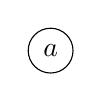
\begin{tikzpicture}[main/.style ={draw,circle}]
            \node[main](a) {$a$};
        \end{tikzpicture}
        \label{fig:internalpair}
    \end{figure}

    Step 9-11: if $\Pi^e\cup \Pi_1=\emptyset$ , either we have already found all external path in this partition or there was none. 
    Either way all terminal pairs left is internal so and $\Pi =\Pi_2$. So we are only interesten in finding the internal path of the internal pairs, which is why we can call $\mathcal{M}$ on each house for itself.
    Each $K_i$ could be a big graph in itself that is decomposable with at least some house $H_i$ where $|H_i|\geq 2$, if this is not the case the algorithm returns after step 3: and continue with the next. 
    If $\mathcal{M}$ has already found some external paths $F$ might not be empty  and may use some arcs inside $K_i$ therefore $F\cap A(K_i)$. $\Pi \cap K_i$ is becouse we are not interested in the terminal pairs that are not a part of the graph we are looking at (pairs inside $K_j$ where $j\neq i$).

    Step 12: Looking for external paths in a big graph is a bit more deficualt since we do not know which arcs and vertices not to use.
    
    Step 13-14: First we find all the pairs that is internal pairs, we want to link as internal paths, the number of these is $k'_i$ for each $i=1,\dots l$. Then we choose a very specifik size of vertex sets $W_i$ and loop over every choiche of these. These vertex set induces a subdigraph, where we make a possible arc set where inside not containg what is inside $F$ we call these $F_i$ we make these set as big as possible linkage need for the rest of the terminal pairs (those we want to find external paths of$\Pi^e\cup \Pi_1$) the number of those is $k'-k'_i$ since every pair mabey has to go through the house we are looking at.
    
    Step 15-19: For each house we remove all vertices not in the vertex set $W_i$ after removing these vertices we remove all remaining arcs except those arcs in $F_i$.
    This is defined in the algorithm as $D''$. We can show that $D''\in \phi(2k^2)$. First we know that since $D$ is totally decomposable $S\in \phi$ and from \autoref{def:bombproof} and the definition on $D(c)$ we can take $S$ add as many parralelle arcs as we want we only need to blow up $l$ vertices those houses of $D$ that are not clean we know that there is $k'$ terminal pairs and that $k'\leq k$ meaning $l\leq 2k$ these $l$ vertices needs to be blown up and from lemma \autoref{lemma:external} lets say that we want to find $k''\leq k'$ external paths in $D$ ($|\Pi^e \cup \Pi_1|=k''$) then we are only looking at $k''$ terminals meaning in every blow up we need at most $2k''(k''+(k-k'))$ since $k''\leq k'$ we have $2k''(k''+(k-k'))\leq 2k''k$ vertices in $W_i$ and $2kk''\leq 2kk'\leq 2k^2$ which is the biggest number we will need to blow up the $l$ vertices meaning $c=2k^2$ so $D''\in \phi (2k^2)$.

    Step 20-24: We need to make sure that the tuple $[K_i,k,k'_i,\Pi_2 \cap K_i,F_i\cup(F\cap A(K_i))]$ upholds every condition for every choice of that tuple. 
    Since we are not focusing on loops we know that the max number of arcs is bounded by the max number of vertices $|F_i|\leq 2kk''$ the rest of the terminals is the number of internal pairs which we in the algorithm denote $k'_i$. we know that $k'_i\leq k'-k''$ meaning $k''\leq k'-k'_i$.
    we start calculating the to demands of $F$ in the tuple.
    Note that $d_{(F\cap A(K_i))}(v)=d_{F}(v), \ \forall v\in V(K_i)$ and we also know $d_{F_i}(v)\leq k''$ so
    \begin{align}
        d^+_{F\cup F_i},d^-_{F\cup F_i}\leq k-k' + k'' = k-(k'-k'')\leq k- k'_i \\
        |(F \cap A(K_i))\cup F_i|\leq |F|+|F_i|\leq 2k(k-k') +2kk''\\
        \leq 2k(k-\textcolor{blue}{k'})+2k(\textcolor{blue}{k'}-k'_i)=2k(k-k'_i).
    \end{align}
    Clearly the tuple for $F$ holds forall its conditions.

\begin{figure}
    \centering
    \begin{tikzpicture}
        %\draw [help lines] (0,0) grid (4,4);

        \node (t2) {$t_2$};
        \node[draw=red,fit=(t2) ,inner sep=1.3ex,circle] (inner1) {};
        
        \node[below right = of t2] (invis1) {};
        \node[draw=red,fit=(invis1) ,inner sep=2ex,circle] (inner2) {};

        \node[above right = of invis1] (t3) {$t_3$};
        \node[draw=red,fit=(t3) ,inner sep=0.7ex,circle] (inner3) {};

        \node[above = 2cm of t3] (t6) {$t_6$};
        \node[above = of t6] (s6) {$s_6$};
        \node[draw=red,fit=(t6)(s6) ,inner sep=1ex,ellipse] (inner4) {};
        
        \node[above = 2cm of t2] (s3) {$s_3$};
        \node[above = of s3] (blank) { };
        \node[draw=red,fit=(s3)(blank) ,inner sep=2.4ex,ellipse] (inner5) {};

        \node[draw=red,fit=(inner1)(inner2)(inner3)(inner4)(inner5) ,inner sep=1ex,ellipse] (outer1) {};


        \node[right = 4cm of t6] (s5) {$s_5$};
        \node[below right = of s5] (s7) {$s_7$};
        \node[below left = of s7] (t7) {$t_7$};
        \node[draw=red, fit=(s5)(s7)(t7),inner sep=3ex,ellipse] (Outer) {};

        \node[below = 5.2cm of s7] (s8) {$s_8$};
        \node[left = of s8] (t8) {$t_8$};
        \node[draw=red, fit=(t8)(s8), inner sep=0.7ex,ellipse] (inner6) {};
        \node[below = of s8] (invis2) {};
        \node[draw=red, fit=(invis2), inner sep=0.7ex,ellipse] (inner7) {};
        \node[left = of invis2] (invis3) {};
        \node[draw=red, fit=(invis3), inner sep=0.7ex,ellipse] (inner8) {};
        \node[draw=red, fit=(inner6)(inner7)(inner8), inner sep=0.2ex,ellipse] (innerout1) {};
        \node[below left = 2.4cm of t8] (invis4) {};
        \node[left = of invis4] (invis5) {};
        \node[draw=red, fit=(invis4)(invis5), inner sep=2.4ex,ellipse] (innerout2) {};
        \node[draw=red, fit=(innerout1)(innerout2), inner sep=0.5ex,ellipse] (outer2) {};

        \node[above = 4.5cm of s3] (s2) {$s_2$};
        \node[above right = 2cm of s2] (t1) {$t_1$};
        \node[draw=red, fit=(s2)(t1),ellipse] (outer3) {};
        \node[right = 5cm of t1] (s1) {$s_1$};
        \node[below right = 1.5cm of s1] (t4) {$t_4$};
        \node[below left = 1cm of t4] (t5) {$t_5$};
        \node[above left= 0.5cm of t5] (s4) {$s_4$};
        \node[draw=red, fit=(s1)(t4)(t5)(s4), inner sep=0.5ex,ellipse] (outer4) {};
        %\node[below right = of ] (invis1) {$t_3$};
        %\node (t3) {$t_3$};
        %\node[below right = of outer1,draw=red,double,fit=(t3) ,inner sep=1ex,circle] (outer2) {};

        %\node [above right = of none] (z){mussi};
    \end{tikzpicture}
    \caption{Example for the algorithm $\mathcal{M}$.}
    \label{fig:mainexample}
\end{figure}
\begin{example}
    This exaple  is based on \autoref{fig:mainexample}.
    The whole figure is considered one digraph $D$ and the set $\Pi = \lbrace (s_1,t_1),\dots ,(s_8,t_8)\rbrace$.
    $D$ is totally $\phi$-decomposable and contain a $\Pi$-linkage. 
    Step 4 gives the houses that is the outer red circles in the figure. 
    Since the decomposition is not trival $D'=D$ we look for clean houses for which there are non. So after step 8 we split $\Pi$ up to external pairs $\Pi^e=\lbrace (s_1,t_1),(s_2,t_2),(s_5,t_5)\rbrace$ and internal pairs $\Pi^i=\lbrace (s_3,t_3), (s_4,t_4), (s_6,t_6),(s_7,t_7),(s_8,t_8)\rbrace$. 
    In this example the partition of the internal pairs is going to be focused on internal paths before external path, meaning $\Pi_1=\emptyset$ first than all set combination of one pair than two pairs and so on.
    So first we have $\Pi_1=\emptyset$ and $\Pi_2=\Pi^i$
    Since $\Pi^e\cup \Pi_1\neq \emptyset$ we enter the if statement in step 14. 
    Then we make the vertex sets $W_i$ which we do not go deep into in this example.\\ 
    Lets say that that we succesfully link the external paths and we now call $\mathcal{M}$ recursively on each house starting with the house in the upper left corner.
    Since we have linked the pairs that was present in this house $\Pi=\emptyset$ and we return. 
    The algorithm now calls itself recursively on the house in the upper right corner.
    Let say this house $H_2\in \phi$ since there are two external terminals in house originally $F$ is properly not empty but it does not matter since we call $\mathcal{B}_{\phi}^-$ that account for this.
    In this case $\mathcal{B}_{\phi}^-$ succesfully link the pair $(s_4,t_4)$.  
    The next house will be the one right under, lets say that the decomposition of this is also trivial but $\mathcal{B}_{\phi}^-$ finds no paths, meaning the algorithm return and make a new partition $\Pi_1=\lbrace (s_3,t_3) \rbrace$ and the rest in $\Pi_2$ but since there is no difference when it comes to the house $H_3$ so the algorithm end up  returning agian making a new partition $\Pi_1=\lbrace (s_4,t_4) \rbrace$ and $\Pi_2=\lbrace (s_3,t_3),(s_6,t_6),(s_7,t_7),(s_8,t_8)\rbrace$. 
    All the external pairs are linked including the pair $(s_4,t_4)$ we call the 3 first houses and like before exept now $H_3$ has no terminals that need to be linked so we return and continue with the house to the left.\\
    $H_4$ has unliked terminals and the $\phi$-decomposition is not trivial, we see the houses clear from the \autoref{fig:mainexample}. The green house is a clean house and so is the house contaning $t_2$ since it is already linked we therefore in step 8 we contract these two sets. 
    In step 9 we split the pairs into external and internal pairs $\Pi^e=\lbrace(s_3,t_3)\rbrace$ and $\Pi^i=\lbrace (s_6,t_6)\rbrace$, So agin since $\Pi^e\cup \Pi_1\neq \emptyset$.
    So we enter the if statement in step 14 link the enternal pair and then call recursively on the houses in except the ones we have contracted either we end up linking the pair internal or ruturn and link it external. 
    We return all the way to the main digraph an call $\mathcal{M}$ on the last house this is not a trival decomposition and there is only an internal pair no external pairs, we contract the green house and instead of entering the if statement in step 14 we enter the if statement in step 11. 
    In this if statement there is no construction of anything and we directly call $\mathcal{M}$ recursive on the house, there is only one and this house does not have a trivial decomposition we contract the two green clean houses and enter the if statement at step 11 since $\Pi_1=\emptyset$ and $\Pi_2=\lbrace (s_8,t_8)\rbrace$   
    It turns out that there only is a $t_8s_8$-path but no $s_8t_8$-path so we return and make a new partition  $\Pi_1=\lbrace (s_8,t_8)\rbrace$ and $\Pi_2=\emptyset$ and enter step 14 instead and we end up linking the piar external. \\
    We enter step 27 and return and enter step 27 and return and now we are at the main digraph enter step 27 and output that a linkage exists. 
\end{example}
\begin{proof}
    We have now proved and explained each step in the algorithm, that it does what we think. 
    Now we need to check whether given your favorite digraph, that upholds the conditions, the algorithm gives the right result.
    If the digraph do not terminate before examine list $\Pi^e\cap \Pi_1$ of $k''$ terminal pairs if $k''=0$ we enter step 9 and $F_i=\emptyset, \text{ for } i=1,\dots l$, and by the induction hypothesis we can assume that if there exists a weak linkage in each $K_i$ the algorithm would find it. 
    Now if this is not the case and $k''>0$ step 12 is then entered and we construct $D''$ which we have described belong to $\phi(2k^2)$ and then as descirbed before we can use $B_\phi^-$ which is correct by \autoref{def:bombproof}, so the algorithm will find a weak $\Pi''$-linkage if it exists in $D''\backslash F'$. 
    After all this there is made a recursiv call on each $K_i$ finding $k'_i$ weak linkages and by the above proof we know it works. 
    So since $B_\phi^-$ correctly finds the weak linkage inside $D''\backslash F'$ using only arcs from $F_i$ $\forall i\in[l]$, then each $K_i$ is recursively called from $D''$ we can easily come back to $D'$ since we find the weak $k'_i$-linkage inside each $K_i$ which is not using any of the arcs from $F_i$ we know that together these stil form the seperated weak linkages.
    By \autoref{lemma:deletarcs} we know that we can find a weak linkage in $D\backslash F$ if we can find it in $D''\backslash F'$ which just proved we can. 
    Given a perfekt weak $\Pi$-linkage.\\
\end{proof}

\subsection{$k$-linkage problem for quasi-transitive digraphs}
We have already establish in \autoref{sec:quasi} that quasi-transitive digraphs are totally $\phi_1$-decomposable.
It turns out that we just have to prove that $\phi_1$ is bombproof, for that we need the two polynomial algorithms $\mathcal{A}_{\phi_1}$ and $\mathcal{B}_{\phi_1}$. Recall that $\phi_1$ is bulid up by semicomplete and acyclic digraphs so we need to establish some theorems for the weak $k$-linkage problem on semicomplete and acyclic digraphs.
\begin{thm}
    The weak $k$-linkage problem is polynomial solvable for every fixed $k$ when the input ia an acyclic digraph.
\end{thm}
\begin{thm}
    The weak $k$-linkage problem polynomial for every fixed $k$, when we consider digraphs that are obtained from a semicomplete digraph by replacing some arcs with multiple copies of those arcs and adding any number of loops.
\end{thm}

Since the bombproof class alows the digraph to no longer be a part of that class we need to consider that an acyclic digraph can get a cycle when blowing up a vertex. 
\begin{thm}
    For every natural number $p$ the weak $k$-linkage problem is polynomial for every fixed $k$, when we consider digraphs with most $p$ directed cycles.
    \label{thm:cycleklink}
\end{thm}
% This is a direct consequence of 
%\begin{thm}
%    For every natural number $\theta$ the weak $k$-linkage problem is polynomial for every fixed $k$, when we consider digraphs with cutwidth at most $\theta$.
%\end{thm}

Now we can prove that $\phi_1$ is bombproof and therefore that quasi-transitive digraphs have a polynomial solution for the weak $k$-linkage problem, when $k$ is fixed.

\begin{thm}
    The class $\phi_1$ is bombproof.
    \label{thm:phi1bomb}
\end{thm}
\begin{proof}
    For $\phi_1$ to be bombproof it has to adhere the properties of \autoref{def:bombproof}, the totally $\phi_1$-decomposition can be found in polynomial time for any $\phi_1$-decomposable digraph by \autoref{thm:phipoly}.
    Now we only need the algorithm $\mathcal{B}_{\phi_1}$ for this we need to look at the constructin of $D(c)$ where $D\in \phi_1$.
    Let $D'\in D(c)$ Either $D$ is semicomplete or $D$ is acylic.\\
    If $D$ is semicomplete $D'$has at most $c$ blown-up vertices $H_1,\dots H_c$ of $D$ to size at most $c$.
    If these $H_i$ is independent we need for each $H_i$ to be semicomplete not need more then $c^2$ arcs. 
    So there is at most $c^3$ arcs missing from $D'$ for it to be semicomplete, then by \autoref{lemma:deletarcs} we can find a weak $k$-linkage for $D'$ if $D$ is semicomplete.
    Now suppose $D$ is acyclic blowing up $c$ vertices with at a size at most $c$, inside these houses of the acyclic digraph there can be no more than $O(c^c)$ cycles pressent in the house.
    Since $D$ is acyclic there is no cycles between the hoouses. 
    There is at most $k$ parallel arcs since no more is needed. which brings up the number of cycles in the house to $O((ck)^c)$ so there is at most $O(c\cdot (ck)^c)$ cycles in $D'$. 
    Then we can use \autoref{thm:cycleklink} where we let $p=c\cdot (ck)^c$.
    So for alll posibilitys of $D$ and all cases of $D'\in D(c)$ we have a pollynomial algorithm that solves the $k$-linkage problem meaning the $\mathcal{B}_{\phi_1}$ algorithm exists and $\phi_1$ is a bombproof class.
\end{proof}



\section{Solving Weak-Linkgae in Locally Semicomplete Digraphs}
\label{sec:wLocally}
Locally semicomplete digraph can be round-decomposable it turns out that we can from the independece number $\alpha (D)$ tell wether a digraph is round-decomposable or not.
Recall independence number from \autoref{sec:digraph}. The theorem below is from \cite{bangJGT77} where we omits some part of it since we have it statet elsewhere in the thises.
\begin{thm}~\cite{bangJGT77}
    A locally semicomplete digraph $D$ havinng idependece number $\alpha (D)$ at least 3 is round decomposable with a unique round -decomposition. 
    \label{thm:independenceround}
\end{thm} 
This means when considering all other locally semicomplete digraphs it has an independence number $\alpha (D) \leq 2$ which means for all not round-decomposable locally semicomplete digraphs we can use the algorithm in \autoref{thm:independencepoly} to solve the weak $k$-linkage problem when $k$ is fixed.
\begin{thm}
        For every natural number $\alpha$ the weak $k$-linkage problem is polynomial for every fixed $k$, when we consider digraphs with independence number at most $\alpha$.
    \label{thm:independencepoly}
\end{thm}
For solving the weak $k$-linkage problem in locally semicomplete digraphs we now only need to find a polynomial algorithm for the round-decomposable once.
Before going into this we have to introduce something called the cutwitdh. This definition of cutwidth is inspired by the describtion of the cutwitdh in \cite{bangJGT77}.\\
Given a digraph $D$ and an ordering of the vertices $O=v_1,\dots,v_n$ we say that the ordering $O$ has a \textbf{cutwidth} at most $\theta$ if $\forall j\in {2,3, \dots n}$ there are at most $\theta$ arcs $u,v$ with $u\in \lbrace v_1,\dots ,v_{j-1}\rbrace$ and $v\in \lbrace v_j,\dots ,v_n\rbrace$ 
\textcolor{red}{inset figur som viser cutwitdh $\theta$ for givet ordering}.
Say we have another ordering $O'$of the same digraph $D$, if $O'$ has a cutwitdh at most $\theta$ for all possible orderings $O'$ of $D$, then $D$ is said to have a \textbf{cutwidth} at most $\theta$. \\
The minimum natural number $\theta$ such that $D$ has a cutwidth at most $\theta$, we call $\theta$ \textbf{the cutwidth} of $D$.
When we know the cutwidth of the digraph we can solve the weak $k$-linkage problem for those i polynomial time.
\begin{thm}~\cite{bangJGT77}
    For every natural number $\theta$ the weak $k$-linkage problem is polynomial for every fixed $k$, when we consider digraphs with cutwidth at most $\theta$.
\end{thm}
\textcolor{red}{introduction to $D_{\Pi}$(side 102 and 104 in \cite{bangJGT77}) + introduce $\Theta$}
\begin{lemma}
    Let $B$ be a digraph of the form $B=R[H_1,\dots H_r]$, where $R$ is round and has cutwidth at least $\Theta$. Let $\Pi$ be a list of piars of terminals. $B$ has a $\Pi$-linkage if and only if $B_\Pi$, has a $\Pi$-linkage.
\end{lemma}
Now we can use all this to prove that $\phi_2$ which is defined in \autoref{sec:gdecomposable} is bombproof and recall that round-decomposable digraphs is totally $\phi_2$-decomposable.
\begin{lemma}
    The class $\phi_2$ is bombproof
\end{lemma}
\begin{proof}
    \textcolor{red}{blablablabalablaba}
\end{proof}
As mensioned above and proved in \autoref{sec:locally} round-decomposable digraphs is totally $phi_2$-decomposable and we have just proved that $\phi_2$ is bombproof so by the algortihm \autoref{alg:weakphi} for bombproof classes every round-decomposable digraph now have a polynomial algorithm to solve the weak $k$-linkage problem.
\begin{thm}
    For every fixed $k$ there exists a polynomial algorithm for the weak $k$-linkage problem for round-decomposable digraphs.
\end{thm}
This ends the part for round-decomposable digraph and in the begining of this section we proved that all other locally semicomplete digraphs than the round-decomposable once have a polynomial algorithm for the weak $k$-linkage problem. We can now state this.
\begin{thm}
    For every fixed $k$ there exists a polynomial algorithm for the weak $k$-linkage problem for locally semicomplete digraphs.
\end{thm}

